\documentclass[a4paper, 12pt]{article}
\usepackage[utf8]{inputenc}
\usepackage[T1]{fontenc}
\usepackage[ngerman]{babel}
\usepackage{geometry}
\usepackage{listings}
\usepackage{xcolor}
\usepackage{hyperref}
\usepackage{helvet}
\usepackage{titlesec}
\usepackage{setspace}
\usepackage{graphicx}
\usepackage{pdfpages}
\usepackage{fancyhdr}
\usepackage{float}
\usepackage{enumitem}
\usepackage{tikz}

\lstdefinelanguage{JavaScript}{
    keywords={break, case, catch, continue, debugger, default, delete, do, else, finally, for, function, if, in, instanceof, new, return, switch, this, throw, try, typeof, var, void, while, with},
    keywordstyle=\color{blue}\bfseries,
    ndkeywords={class, const, enum, export, extends, import, super, implements, interface, let, package, private, protected, public, static, yield, null, true, false},
    ndkeywordstyle=\color{darkgray}\bfseries,
    identifierstyle=\color{black},
    sensitive=false,
    comment=[l]{//},
    morecomment=[s]{/*}{*/},
    commentstyle=\color{purple}\ttfamily,
    stringstyle=\color{red}\ttfamily,
    morestring=[b]',
    morestring=[b]"
}

\lstset{
    language=JavaScript,
    extendedchars=true,
    basicstyle=\footnotesize\ttfamily,
    showstringspaces=false,
    showspaces=false,
    numbers=left,
    numberstyle=\footnotesize,
    numbersep=9pt,
    tabsize=2,
    breaklines=true,
    showtabs=false,
    captionpos=b
}
\geometry{a4paper, left=2.5cm, right=2.5cm, top=3cm, bottom=3cm, headsep=1.5cm}

\setlength{\parindent}{0pt}
\setlength{\parskip}{6pt}
\graphicspath{ {./images/} }

\pagestyle{fancy}
\fancyhf{}
\rhead{\vspace{0.2cm}
\includegraphics[width=4cm]{hs_mainz_logo}}
\fancypagestyle{plain}{
    \fancyhf{}
    \rhead{\vspace{0.2cm}
\includegraphics[width=4cm]{hs_mainz_logo}}
}
\renewcommand{\headrulewidth}{0pt}
\renewcommand{\footrulewidth}{0pt}
\fancyfoot[C]{\thepage}

\newcounter{lastroman}
\newrobustcmd{\switchtopage}[1]{
    \clearpage
    \setcounter{lastroman}{\value{page}}
    \pagenumbering{#1}
}
\newrobustcmd{\switchback}{
    \clearpage
    \pagenumbering{Roman}
    \setcounter{page}{\value{lastroman}}
}

% Document
\begin{document}

    \begin{titlepage}
    \centering
    \vspace*{1cm}

    
\includegraphics[width=0.4\textwidth]{hs_mainz_logo}\\
    \vspace{1.5cm}

    \textbf{\LARGE Praxismodul I}\\
    \vspace{0.5cm}
    \textbf{\Large Collectiqo}\\
    \vspace{1.5cm}

    \textbf{Hochschule Mainz}\\
    \vspace{0.5cm}
    Fachbereich Wirtschaft\\
    \vspace{0.5cm}
    B.Sc. Wirtschaftsinformatik dual\\
    \vspace{1.5cm}

    \textbf{Authors:}\\
    Bindernagel, Lorenz\\
    Schäfer, Robin\\
    Šimić, Darko\\
    Struve, Anika\\
    \vfill

    \today
\end{titlepage}

    % \maketitle
    \newpage
    \tableofcontents
    \newpage

    \section{Projektidee und Konzept}\label{sec:idee-konzept}
    \subsection{Motivation}\label{subsec:Motivation}
Das Sammeln von Kulturgütern ist ein Bedürfnis von vielen verschiedenen Menschen und eine faszinierende Praxis, die tiefe Einblicke in Geschichte, Identität und ästhetische Vorlieben gewährt.
Es ist eine Leidenschaft, die Menschen verschiedener Hintergründe und Interessen verbindet, sei es das Sammeln von Parfumflaschen, Videospielen oder historischen Münzen.
Diese vielfältigen Sammlungen zeugen von der menschlichen Neugierde und dem Bedürfnis, materielle Kulturgüter zu bewahren und zu schätzen. \par

Trotz des reichen Angebots an Online-Plattformen zur Verwaltung einzelner Sammlungen fehlt allerdings bisher eine universelle Plattform, die es ermöglicht, mehrere Sammlungen unterschiedlicher Genres unter einem einheitlichen Dach zu pflegen und zu dokumentieren.
Das Praxisprojekt namens Collectiqo strebt danach, diese Lücke zu füllen, indem sie eine ansprechende und zugängliche Plattform bietet, um diverse Sammlungen zu organisieren, zu dokumentieren und zu präsentieren, unabhängig von deren thematischer Ausrichtung.


\subsection{Marktanalyse / Technologische Grundlagen}\label{subsec:Marktanalyse-TechnologischeGrundlagen}
Zielgruppe, Marktabgrenzung, theoretische Grundlagen, Literaturüberblick\linebreak
Design Science: Relevance-Cycle
    \newpage


    \section{Projektplanung und Projektmanagement}\label{sec:planung-management}
    \subsection{Zieldefinition}\label{subsec:Zieldefinition}
Das Ziel dieses Projekts ist die Entwicklung und Implementierung einer universellen Sammlerplattform, die es Benutzern ermöglicht, ihre Sammlungen digital zu verwalten, zu präsentieren und mit anderen zu teilen.
Diese Plattform soll benutzerfreundlich, flexibel und skalierbar sein, um eine breite Palette von Sammlerbedürfnissen abzudecken.

% Wir könnten hier sicherlich auch das Wording Meilensteine nutzen, finde ich besser als Teilergebnisse
\subsection{Teilergebnisse}\label{subsec:Teilergebnisses}
Die Teilergebnisse lassen sich aus dem Konzept in ~\ref{subsec:Designphase} ableiten.
Grundlegende Teilergebnisse sind die Erstellung des Frontends, die Erstellung des Backends und die Einrichtung einer Datenbank.
Neben diesen Zielen, die sich aus der verwendeten Architektur ergeben, ist ein weiteres Teilergebnis das Hosting der Website und der Datenbank.
Für jedes Teilergebnis sind Voranalysen notwendig, da die Programmierung einer Webanwendung für das gesamte Team neu ist.
Als Ausgangspunkt für die Analyse diente GitHub Eduction, das mit dem Kurs Intro to Web Development einige Tools für die Entwicklung von Websites zur Verfügung stellt.
Die in der Analyse ausgewählten Tools sind in ~\ref{subsec:Tools} aufgelistet.

Die Teilergebnisse sind eng miteinander verknüpft.
Das Hosting der Website und der Datenbank sind von entscheidender Bedeutung.
Insbesondere das Backend ist ohne die Datenbank nur schwer zu entwickeln.
Das Hosting der Website ist wichtig, um die integrierten Funktionen direkt live testen zu können.
Die Entwicklung von Frontend, Backend und Datenbank ist eng miteinander verzahnt.
Frontend und Datenbank lassen sich separat einrichten, das Backend ist für die Kommunikation der beiden Bereiche unerlässlich.
Während die drei Bereiche einzelne Teilergebnisse darstellen, erfolgt der Großteil der Programmierung parallel.

Das Frontend ist alles, womit der Benutzer letztendlich auf der Website interagieren kann.
Beispiele hierfür sind die Login-Seite, die Ansicht der verschiedenen Sammlungen und die Seite zur Erstellung von Vorlagen.
Im Anhang finden sich Mockups, die während des anfänglichen Brainstormings der Projektidee entstanden sind.
Das Backend ist für die Kommunikation zwischen dem Frontend und der Datenbank verantwortlich.
Es soll die Daten aus der Datenbank an das Frontend zur Anzeige weiterleiten.
Außerdem soll es Änderungen an den Daten, die in der Benutzeroberfläche vorgenommen werden, an die Datenbank kommunizieren.
Dabei ist es wichtig, dass die Funktionen sicherstellen, dass die Datenbank dynamisch auf Basis der Benutzereingaben skaliert wird.
Die Logik der Website sollte in diesem Teil des Programms definiert werden.
Das Datenbanksystem ist der Ort, an dem Informationen über Benutzer und Sammlungen gespeichert werden.
Die Datenbankform der Sammlungsvorlagen wird hier gespeichert.
Es muss so konfiguriert sein, dass das dynamische Hinzufügen und Löschen ganzer Tabellen möglich ist.
% Vllt mal ein Mockup für ein Template erstellen

\subsection{Definitions of done}\label{subsec:DoD}
Im Rahmen des Projekts wurden die folgenden Definitions of Done festgelegt, um den erfolgreichen Abschluss der verschiedenen Projektaufgaben und -phasen sicherzustellen:

\begin{enumerate}
\item \textbf{Die Idee des Projektes ist erstellt:}
\begin{itemize}[label=--, itemsep=0pt, parsep=0pt]
\item Eine klare und detaillierte Beschreibung des Projektziels und der Motivation liegt vor.
\item Das Projektziel ist verständlich und umfassend dokumentiert.
\end{itemize}

\item \textbf{Auswahl der genutzten Software- bzw. Projektwerkzeuge ist erfolgt:}
\begin{itemize}[label=--, itemsep=0pt, parsep=0pt]
\item Alle notwendigen Software- und Projektmanagement-Tools sind ausgewählt und dokumentiert.
\item Die Gründe für die Auswahl der jeweiligen Werkzeuge sind festgehalten.
\end{itemize}

\item \textbf{Projektplanung ist angelegt:}
\begin{itemize}[label=--, itemsep=0pt, parsep=0pt]
\item Ein detaillierter Projektplan mit Zeitplan, Meilensteinen und Ressourcenplanung ist erstellt.
\item Der Projektplan ist mit dem Projektteam abgestimmt und genehmigt.
\end{itemize}

\item \textbf{Erstellung von Konzept und Projektplan (Abgabe 1) erfolgreich und genehmigt:}
\begin{itemize}[label=--, itemsep=0pt, parsep=0pt]
\item Das Konzept und der Projektplan sind fertiggestellt und den entsprechenden Gremien oder Betreuern vorgelegt.
\item Eine formelle Genehmigung oder Freigabe wurde erteilt.
\end{itemize}

\item \textbf{Anlegen der Projektumgebung mithilfe der Software- bzw. Projektwerkzeuge erfolgte:}
\begin{itemize}[label=--, itemsep=0pt, parsep=0pt]
\item Die Projektumgebung ist vollständig eingerichtet, einschließlich aller erforderlichen Software- und Hardwarekomponenten.
\item Alle Teammitglieder haben Zugang und die notwendige Schulung für die genutzten Werkzeuge erhalten.
\end{itemize}

\item \textbf{Backend-System ist implementiert:}
\begin{itemize}[label=--, itemsep=0pt, parsep=0pt]
\item Das Backend-System ist vollständig entwickelt und funktionsfähig.
\item Alle geplanten Funktionen und Schnittstellen sind implementiert und getestet.
\end{itemize}

\item \textbf{Frontend-System ist implementiert:}
\begin{itemize}[label=--, itemsep=0pt, parsep=0pt]
\item Das Frontend-System ist vollständig entwickelt und funktionsfähig.
\item Das Design entspricht den vorher festgelegten Spezifikationen und ist benutzerfreundlich.
\end{itemize}

\item \textbf{Datenbanksystem ist implementiert:}
\begin{itemize}[label=--, itemsep=0pt, parsep=0pt]
\item Die Datenbank ist eingerichtet, strukturiert und alle notwendigen Tabellen und Beziehungen sind vorhanden.
\item Die Datenbank erfüllt die Anforderungen hinsichtlich Performance und Sicherheit.
\end{itemize}

\item \textbf{Verknüpfung der drei Systeme erfolgte:}
\begin{itemize}[label=--, itemsep=0pt, parsep=0pt]
\item Backend, Frontend und Datenbanksystem sind nahtlos integriert.
\item Die Kommunikation zwischen den Systemen ist getestet und funktioniert einwandfrei.
\end{itemize}

\item \textbf{Account-Erstellung und Benutzer-Login ist möglich:}
\begin{itemize}[label=--, itemsep=0pt, parsep=0pt]
\item Nutzer können erfolgreich Accounts erstellen und sich in das System einloggen.
\item Die Authentifizierungsmechanismen sind sicher und funktionieren zuverlässig.
\end{itemize}

\item \textbf{Vorhandene „Sammlungen“-Templates können genutzt werden:}
\begin{itemize}[label=--, itemsep=0pt, parsep=0pt]
\item Standard-Templates für Sammlungen sind verfügbar und können von den Benutzern angewendet werden.
\item Diese Templates sind funktional und ansprechend gestaltet.
\end{itemize}

\item \textbf{Benutzer kann erfolgreich eigene Templates anlegen:}
\begin{itemize}[label=--, itemsep=0pt, parsep=0pt]
\item Nutzer haben die Möglichkeit, eigene Templates für ihre Sammlungen zu erstellen und zu speichern.
\item Die Anpassung und Nutzung dieser Templates ist intuitiv und problemlos möglich.
\end{itemize}

\item \textbf{Benutzerrechte-Einstellungen sind passend:}
\begin{itemize}[label=--, itemsep=0pt, parsep=0pt]
\item Benutzerrechte und -rollen sind definiert und korrekt implementiert.
\item Die Plattform stellt sicher, dass Benutzer nur auf die ihnen zugewiesenen Bereiche und Funktionen zugreifen können.
\end{itemize}

\item \textbf{Alle notwendigen Tests erfolgreich:}
\begin{itemize}[label=--, itemsep=0pt, parsep=0pt]
\item Alle geplanten Tests (Unit-Tests, Integrationstests, Systemtests, Usability-Tests) sind abgeschlossen.
\item Die Testergebnisse sind dokumentiert und alle kritischen Fehler sind behoben.
\end{itemize}

\item \textbf{Projektdokumentation ist erstellt:}
\begin{itemize}[label=--, itemsep=0pt, parsep=0pt]
\item Eine vollständige und detaillierte Dokumentation des Projekts ist vorhanden.
\item Die Dokumentation umfasst alle Aspekte der Entwicklung, Implementierung und Nutzung der Plattform.
\end{itemize}

\item \textbf{Produktpräsentation fertiggestellt:}
\begin{itemize}[label=--, itemsep=0pt, parsep=0pt]
\item Eine umfassende Produktpräsentation ist vorbereitet, die alle wichtigen Funktionen und Vorteile der Plattform darstellt.
\item Die Präsentation ist auf die Zielgruppe abgestimmt und beinhaltet anschauliche Beispiele und Demonstrationen.
\end{itemize}

\item \textbf{Projektbericht + Präsentation (Abgabe 2) erfolgreich und abgenommen:}
\begin{itemize}[label=--, itemsep=0pt, parsep=0pt]
\item Der abschließende Projektbericht ist fertiggestellt und eingereicht.
\item Die Präsentation wurde erfolgreich durchgeführt und das Projekt wurde offiziell abgenommen.
\end{itemize}
\end{enumerate}


\subsection{Projektstrukturplan}\label{subsec:PSP}
Lorenz ipsum dolor sit amet, consetetur sadipscing elitr, sed diam nonumy eirmod tempor invidunt ut labore et dolore magna aliquyam erat, sed diam voluptua.
At vero eos et accusam et justo duo dolores et ea rebum.
Stet clita kasd gubergren, no sea takimata sanctus est Lorem ipsum dolor sit amet.
Lorenz ipsum dolor sit amet, consetetur sadipscing elitr, sed diam nonumy eirmod tempor invidunt ut labore et dolore magna aliquyam erat, sed diam voluptua.
At vero eos et accusam et justo duo dolores et ea rebum.
Stet clita kasd gubergren, no sea takimata sanctus est Lorem ipsum dolor sit amet.
Lorenz ipsum dolor sit amet, consetetur sadipscing elitr, sed diam nonumy eirmod tempor invidunt ut labore et dolore magna aliquyam erat, sed diam voluptua.
At vero eos et accusam et justo duo dolores et ea rebum.
Stet clita kasd gubergren, no sea takimata sanctus est Lorem ipsum dolor sit amet.

\begin{figure}[H]
    \centering
    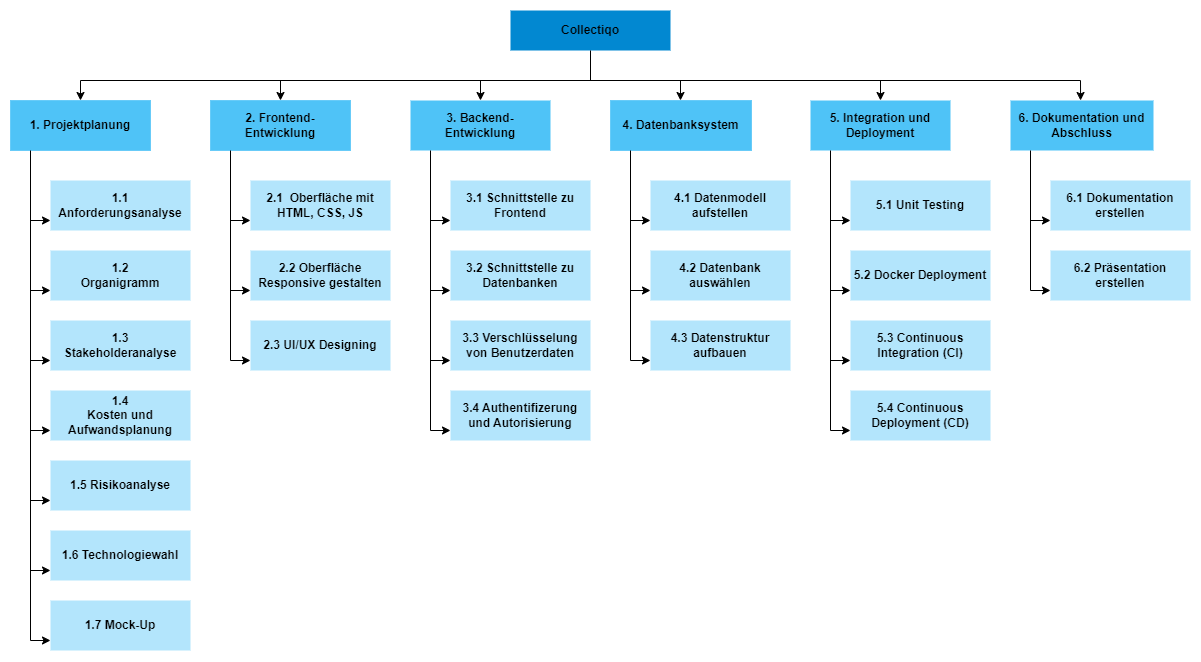
\includegraphics[width=1.0\textwidth]{psp}
    \caption{Projektstrukturplan}
\end{figure}

\subsection{Organigramm}\label{subsec:Organigramm}

\begin{figure}[H]
    \centering
    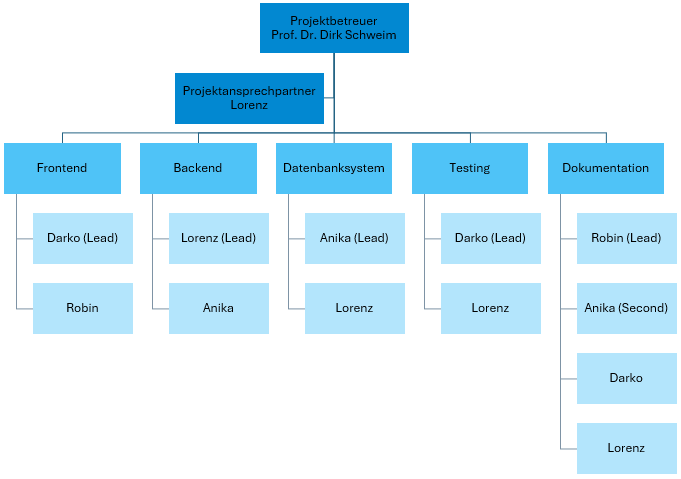
\includegraphics[width=0.8\textwidth]{organigramm}
    \caption{Organigramm}
\end{figure}

Das Organigramm weist die Struktur und die Verantwortlichkeiten innerhalb des Projektteams auf. Es gibt einen klaren Aufbau, der die verschiedenen Rollen und Zuständigkeiten verdeutlicht.

\subsubsection{Projektbetreuer}
\begin{itemize}
    \item \textbf{Prof. Dr. Dirk Schweim:} Der Projektbetreuer steht an oberster Stelle und ist für die Betreuung des Projekts verantwortlich.
\end{itemize}

\subsubsection{Projektansprechpartner}
\begin{itemize}
    \item \textbf{Lorenz:} Der Projektansprechpartner steht direkt unter dem Projektbetreuer und ist für die Koordination und Kommunikation innerhalb des Teams als auch zum Projektbetreuer zuständig.
\end{itemize}


\subsubsection{Frontend}
\begin{itemize}
    \item \textbf{Hauptverantwortlich:} Darko
    \item \textbf{Vertretend:} Robin
\end{itemize}
Die Frontend-Sparte ist für die Gestaltung und Implementierung der Benutzeroberfläche zuständig.
Darko ist hauptverantwortlich für diese Abteilung, unterstützt von Robin.

\subsubsection{Backend}
\begin{itemize}
    \item \textbf{Hauptverantwortlich:} Lorenz
    \item \textbf{Vertretend:} Anika
\end{itemize}
Das Backend kümmert sich um die serverseitige Logik und Datenverarbeitung.
Lorenz ist der Hauptverantwortliche, wobei Anika unterstützend tätig ist.

\subsubsection{Datenbanksystem}
\begin{itemize}
    \item \textbf{Hauptverantwortlich:} Anika
    \item \textbf{Vertretend:} Lorenz
\end{itemize}
Diese Sparte ist für die Verwaltung und Wartung der Datenbank zuständig.
Anika hat die Hauptverantwortung, unterstützt von Lorenz.

\subsubsection{Testing}
\begin{itemize}
    \item \textbf{Verantwortlich:} Darko, Lorenz
\end{itemize}
Testing führt Tests durch, um die Qualität und Funktionalität der Plattform sicherzustellen.
Darko und Lorenz teilen sich die Verantwortung in diesem Bereich.

\subsubsection{Dokumentation}
\begin{itemize}
    \item \textbf{Hauptverantwortlich:} Robin
    \item \textbf{Vertretend verantwortlich:} Anika
    \item \textbf{Weitere Beteiligte:} Darko, Lorenz
\end{itemize}
Die Dokumentation wird von allen im Projektteam erstellt geflegt.
Robin ist hauptverantwortlich, Anika übernimmt eine vertretende Rolle, während auch Darko und Lorenz aktiv mitwirken.

Diese Struktur weist eine klare Rollenverteilung und entsprechende Vertretung auf, die dem Projektteam ermöglicht, effizient und effektiv an Aufgaben zu arbeiten und ermöglicht eine bessere Zusammenarbeit.



\subsection{Ablaufplanung (Gantt / Netzplan)}\label{subsec:Ablaufplan}
Wird in YouTrack erstellt.

Lorenz ipsum dolor sit amet, consetetur sadipscing elitr, sed diam nonumy eirmod tempor invidunt ut labore et dolore magna aliquyam erat, sed diam voluptua.
At vero eos et accusam et justo duo dolores et ea rebum.
Stet clita kasd gubergren, no sea takimata sanctus est Lorem ipsum dolor sit amet.
Lorenz ipsum dolor sit amet, consetetur sadipscing elitr, sed diam nonumy eirmod tempor invidunt ut labore et dolore magna aliquyam erat, sed diam voluptua.
At vero eos et accusam et justo duo dolores et ea rebum.
Stet clita kasd gubergren, no sea takimata sanctus est Lorem ipsum dolor sit amet.
Lorenz ipsum dolor sit amet, consetetur sadipscing elitr, sed diam nonumy eirmod tempor invidunt ut labore et dolore magna aliquyam erat, sed diam voluptua.
At vero eos et accusam et justo duo dolores et ea rebum.
Stet clita kasd gubergren, no sea takimata sanctus est Lorem ipsum dolor sit amet.

\subsection{Stakeholder- und Risikoanalyse}\label{subsec:Stakeholder-Risikoanalyse}
Im Folgenden wurde eine Analyse bezüglich der Stakeholder des Projektes erstellt.
Diese haben unterschiedliche Vorstellungen, Einstellungen und Ansichten zum Projekt.
Diese sind auch in interne und externe Stakeholder eingeteilt, allerdings sollte beachtet werden, dass die Priorität bei internen Stakeholdern liegt, da das Projekt universitär ist.
Ergänzend wurde auch eine Risikoanalyse erstellt, welche zur Übersicht von eventuell eintretenden Problemen verhilft.

%\begin{figure}[h]
%Warum auch immer, der verschiebt die Grafik zwei Punkte weiter wenn figure angewendet wird, schau ich mir später an -Anika
    \centering
    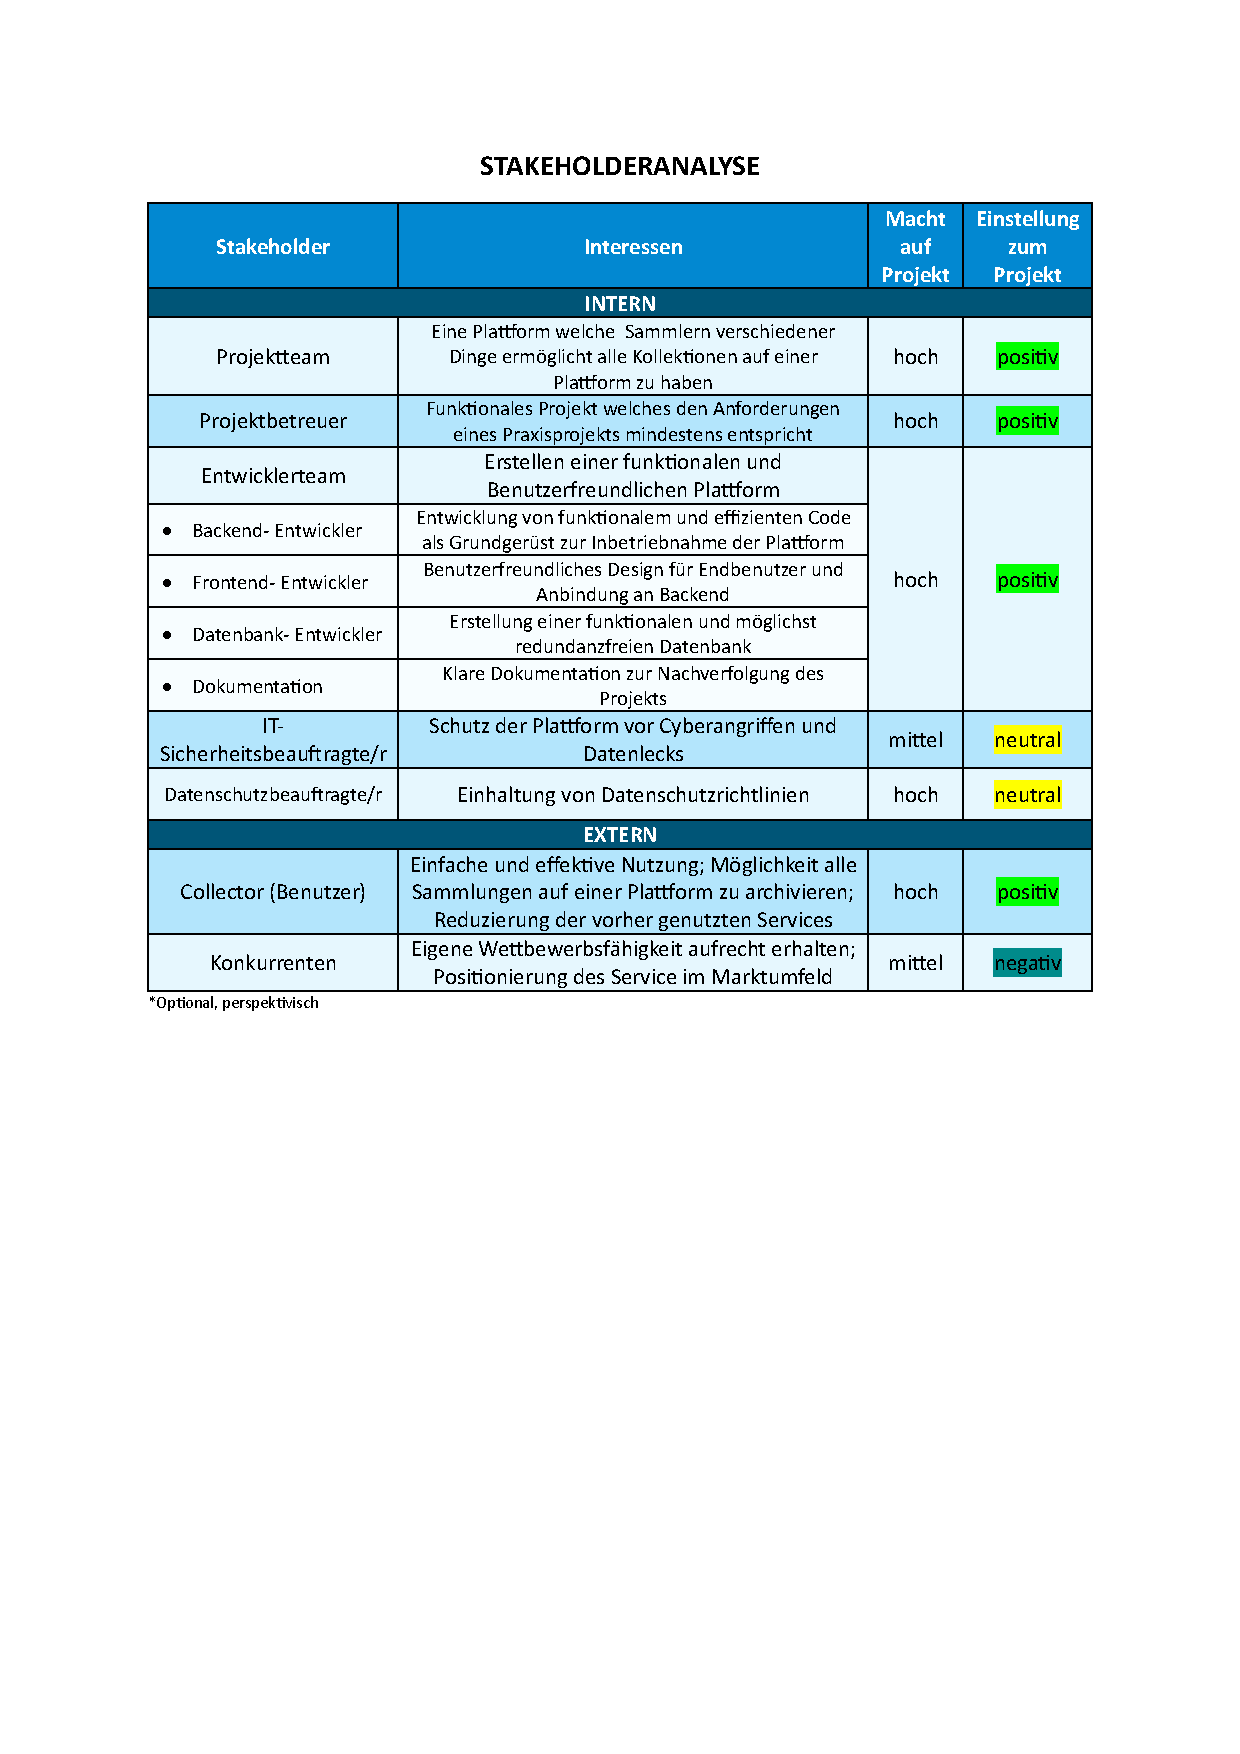
\includegraphics[pages=1, pagecommand={}, width=\textwidth, clip, trim=0cm 12.2cm 0cm 3cm]{PM_SH_RISK_ANALYSIS}
    \caption{Stakeholderanalyse}
%\end{figure}

Das Projektteam besteht aus Studierenden, die im Rahmen ihres Studiums die Plattform entwickeln.
Das Hauptziel des Teams ist analog zur Zieldefinition von ~\ref{subsec:Zieldefinition}.
Rückblickend auf die Motivation in ~\ref{subsec:Motivation} ist das Team positiv eingestellt. \par

Der Projektbetreuer, Herr Prof. Dr. Schweim, hat ein starkes Interesse daran, dass das Projekt den Anforderungen eines praxisnahen Studienprojekts entspricht.
Sein Fokus liegt darauf, dass das Projekt nicht nur funktional, sondern auch innovativ und praxisnah ist.
Er hat erheblichen Einfluss auf den Projektverlauf und unterstützt das Team mit wertvollem Feedback und fachlicher Anleitung. \par

Das Entwicklerteam, welches aus dem Projektteam besteht, ist in mehrere spezialisierte Gruppen unterteilt, analog zum Organigramm in ~\ref{subsec:Organigramm}.
Alle Entwicklergruppen haben parallel zum Projektteam-Stakeholder ein hohes Interesse am Projekterfolg und eine positive Einstellung zur Aufgabe, die einzelnen Interessen wurden zwecks persönlicher Lernerfolge nochmal aufgelistet. \par

Als letzten internen Stakeholder erweist sich die Rolle der Datenschutzbeauftragten, dessen Hauptaufgabe darin besteht, die Einhaltung der Datenschutzrichtlinien sicherzustellen.
Diese Rolle hat einen hohen Einfluss auf das Projekt, da Datenschutz ein wesentliches, aber auch rechtliches Kriterium für die Plattform darstellt.
Entsprechend ist die Einstellung neutral gehalten. \par


Die Hauptnutzer der Plattform, die Sammler (Collector), stellen einen wesentlichen externen Stakeholder dar.
Ihr Interesse liegt in der einfachen und effektiven Nutzung der Plattform, die es ihnen ermöglicht, ihre Sammlungen zentral zu archivieren und die Nutzung mehrerer vorheriger Dienste zu reduzieren.
Ihre hohe Erwartung und positive Einstellung gegenüber der Plattform sind entscheidend für dessen Akzeptanz und Projekterfolg. \par

Auf der anderen Seite stehen die Konkurrenten, die ihre eigene Wettbewerbsfähigkeit wahren und ihre Marktposition behaupten wollen.
Diese Stakeholder können dem Projekt eher negativ gegenüberstehen, da die neue Plattform potenziell eine Bedrohung für ihre eigenen Dienstleistungen darstellt.
Ihr Einfluss ist letztlich niedrig aufgrund des universitären Zwecks des Projektes, dennoch spielen sie einen Faktor bezüglich des Aufbaus und der eigentlichen Motivation der Plattform. \par







\subsection{Kosten- und Aufwandsplanung}\label{subsec:Kosten-Aufwandsplanung}
Lorenz ipsum dolor sit amet, consetetur sadipscing elitr, sed diam nonumy eirmod tempor invidunt ut labore et dolore magna aliquyam erat, sed diam voluptua.
At vero eos et accusam et justo duo dolores et ea rebum.
Stet clita kasd gubergren, no sea takimata sanctus est Lorem ipsum dolor sit amet.
Lorenz ipsum dolor sit amet, consetetur sadipscing elitr, sed diam nonumy eirmod tempor invidunt ut labore et dolore magna aliquyam erat, sed diam voluptua.
At vero eos et accusam et justo duo dolores et ea rebum.
Stet clita kasd gubergren, no sea takimata sanctus est Lorem ipsum dolor sit amet.
Lorenz ipsum dolor sit amet, consetetur sadipscing elitr, sed diam nonumy eirmod tempor invidunt ut labore et dolore magna aliquyam erat, sed diam voluptua.
At vero eos et accusam et justo duo dolores et ea rebum.
Stet clita kasd gubergren, no sea takimata sanctus est Lorem ipsum dolor sit amet.

\subsection{Tools}\label{subsec:Tools}
Lorenz ipsum dolor sit amet, consetetur sadipscing elitr, sed diam nonumy eirmod tempor invidunt ut labore et dolore magna aliquyam erat, sed diam voluptua.
At vero eos et accusam et justo duo dolores et ea rebum.
Stet clita kasd gubergren, no sea takimata sanctus est Lorem ipsum dolor sit amet.
Lorenz ipsum dolor sit amet, consetetur sadipscing elitr, sed diam nonumy eirmod tempor invidunt ut labore et dolore magna aliquyam erat, sed diam voluptua.
At vero eos et accusam et justo duo dolores et ea rebum.
Stet clita kasd gubergren, no sea takimata sanctus est Lorem ipsum dolor sit amet.
Lorenz ipsum dolor sit amet, consetetur sadipscing elitr, sed diam nonumy eirmod tempor invidunt ut labore et dolore magna aliquyam erat, sed diam voluptua.
At vero eos et accusam et justo duo dolores et ea rebum.
Stet clita kasd gubergren, no sea takimata sanctus est Lorem ipsum dolor sit amet.

\begin{itemize}
\item one
\item two
\item three
\end{itemize}


    \newpage


    \section{Projektbericht}\label{sec:projektberichts}
    \subsection{Allgemeine Methodik / Vorgehen / Literaturüberblick}\label{subsec:Methodik}
Bspw.: Business Model Canvas / CRSIP-DM-Cycle / Behavior Driven Development / SCRUM)
Design Science: Rigor-Cycle

\subsection{Designphase}\label{subsec:Designphase}
Datenmodell / Frontend / Backend
Design Science: Design-Cycle

\subsubsection{Backend}
Der erste Schritt bei der Backend entwicklung war es, einen geeigneten Startpunkt zu finden.
Hierbei wurde entschieden, dass zuerst eine Implementierung der Datenbankverbindung erfolgen sollte, da diese als Grundlage für die weitere Entwicklung dient.
Dies wurde mit der Bibliothek mysql2 realisiert, welche eine erweiterte Funktionalität gegenüber der Standardbibliothek bietet und diverse Probleme behebt.
Diese implementierung war erst möglich, nachdem die Grundstruktur der Datenbank aufgesetzt wurde.
Einen Einblick in den Code gibt Listing\ref{lst:dbconnector}.

\lstinputlisting[language=JavaScript,label={lst:dbconnector}]{../server/dbConnector.js}

Als Nächstes wurde sich dazu entschieden, ein einfaches Sign Up und Login System zu programmieren.
Hierbei wurde auf die Bibliothek bcrypt zurückgegriffen, welche das Hashen von Passwörtern erleichtert.
Die SQL queries, die hier genutzt werden, wurden ebenfalls mit der mysql2 Bibliothek realisiert.
Die einzigen Nutzerdaten, die hierbei gespeichert werden, sind der Username, die E-Mail und das Passwort.
Beim Login wurde darauf geachtet, das Nutzer Username und E-Mail benutzen können, um sich einzuloggen.

Nun stellte sich die Frage, wie es möglich ist, dass Nutzer nur auf ihre eigenen Sammlungen zugreifen können.
Beim Recherchieren sind wir auf das Konzept von Sessions gestoßen und wollten diese ausprobieren.

Parallel wurde eine Funktion entwickelt, die Daten aus der Datenbank anhand des Tabellennamens ausliest.
Diese werden dann in eine Form gebracht, welche das Frontend nutzen kann, um Beispieldaten in einer Tabelle einzupflegen.



\subsubsection{Datenbank}

Bei der Einrichtung der Datenbank stellt sich als erste Hürde der Umgang mit Docker Container heraus.
Zwar waren grundlegende Kentnisse über Docker vorhanden, doch eine Datenbank praktisch in einem Container hochzufahren und diese dann mit dem Code und der Programmierumgebung zu verknüpfen, war eine neue Herausforderung.
Hierzu mehr in Kapitel~\ref{subsec:Herausforderungen}.
Wie in der Planung entschieden, sollen zwei Datenbanken genutzt werden - eine MySQL Datenbank für strukturierte Daten und eine MongoDB Datenbank für unstrukturierte Daten.
Im ersten Schritt wurde die MySQL Datenbank aufgesetzt und mit Tabellen für Nutzerdaten und den drei Pre-Sets für Sammlungen befüllt.
Die Nutzerdaten beinhalten Username, E-Mail und Passwort.
Für die Themenbereiche Video Spiele und Parfum wurden jeweils eine Tabelle erstellt, die für das Thema passende Spalten beinhalten.

\subsection{Herausforderungen}\label{subsec:Herausforderungen}

Bei der Programmierung des Projekts gab es einige Stellen, an denen das Team auf Probleme, und vor allem auf steile Lernkurven stieß.
Eine dieser Stellen war der Umgang mit Docker Containern.
Ein gewisses Grundverständnis war vorhanden, doch praktische Erfahrung war im gesamten Team nicht vorhanden.
Zwar was das Hochfahren einer Datenbank in einem Container schnell erreicht, doch ein Verständnis für Datenpersistenz und Volumes zu entwickeln, benötigte seine Zeit.
Auch im späteren Verlauf des Projekts, als es darum ging alle Applikationskomponenten in einer Docker-Compose Datei zusammenzuführen, stellte sich als Herausforderung heraus.
Wie sich Dockerfiles in dem ganzen System einordnen und wo sie genutzt werden, war ebenfalls neu für das Team.
Allgemein hat das Einfinden in Docker dem Team mehr Zeit als erwartet abverlangt.

Eine weitere Herausforderung war das Einfinden in die verschiedenen Bibliotheken, die bei Webentwicklung mit JavaScript genutzt werden.
Zwar wurde in der Planung bereits einige Bibliotheken festgelegt, die genutzt werden sollten, doch während der Entwicklung kamen einige neue hinzu.
Ein Beispiel hierfür ist die Bibliothek express-session, die für das Session-Management genutzt wird.
Da zur Planung noch kein detailliertes Verständnis darüber vorhanden war, welche Komponenten bei der Entwicklung einer solchen Anwendung benötigt werden, wurden Thematiken wie Session Management erst während der Entwicklung entdeckt.
Hierdurch kam es an einigen Stellen zu steilen, jedoch unvermeidbaren Lernkurven.

\subsection{Prototypvorstellung}\label{subsec:Prototyp}
Design Science: Artefakt
    \newpage


    \section{Ergebnis und Fazit}\label{sec:ergebnis-fazit}
    \subsection{Fazit}\label{subsec:Fazit}

\subsection{Lessons learned}\label{subsec:LessonsLearned}

\subsection{Ausblick}\label{subsec:Ausblick}

Lorem ipsum dolor sit amet, consetetur sadipscing elitr, sed diam nonumy eirmod tempor invidunt ut labore et dolore magna aliquyam erat, sed diam voluptua.
At vero eos et accusam et justo duo dolores et ea rebum.
Stet clita kasd gubergren, no sea takimata sanctus est Lorem ipsum dolor sit amet.
Lorem ipsum dolor sit amet, consetetur sadipscing elitr, sed diam nonumy eirmod tempor invidunt ut labore et dolore magna aliquyam erat, sed diam voluptua.
At vero eos et accusam et justo duo dolores et ea rebum.
Stet clita kasd gubergren, no sea takimata sanctus est Lorem ipsum dolor sit amet.
    \newpage

    \appendix


    \section{Anhang}\label{sec:anhang}
    \subsection{Mockups}\label{subsec:Mockups}

\begin{figure}[htbp]
    \centering
    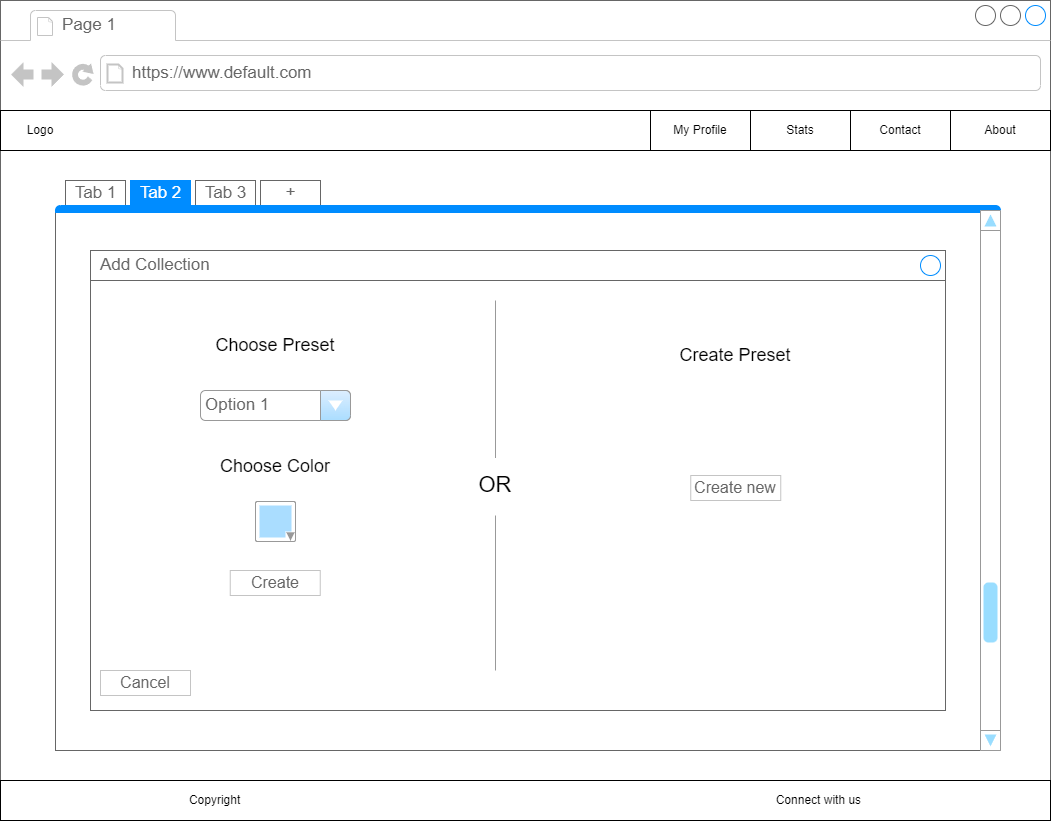
\includegraphics[width=0.6\textwidth]{add_collection_pop_up}
    \caption{'Add Collection' Pop-up}
\end{figure}

\begin{figure}[htbp]
    \centering
    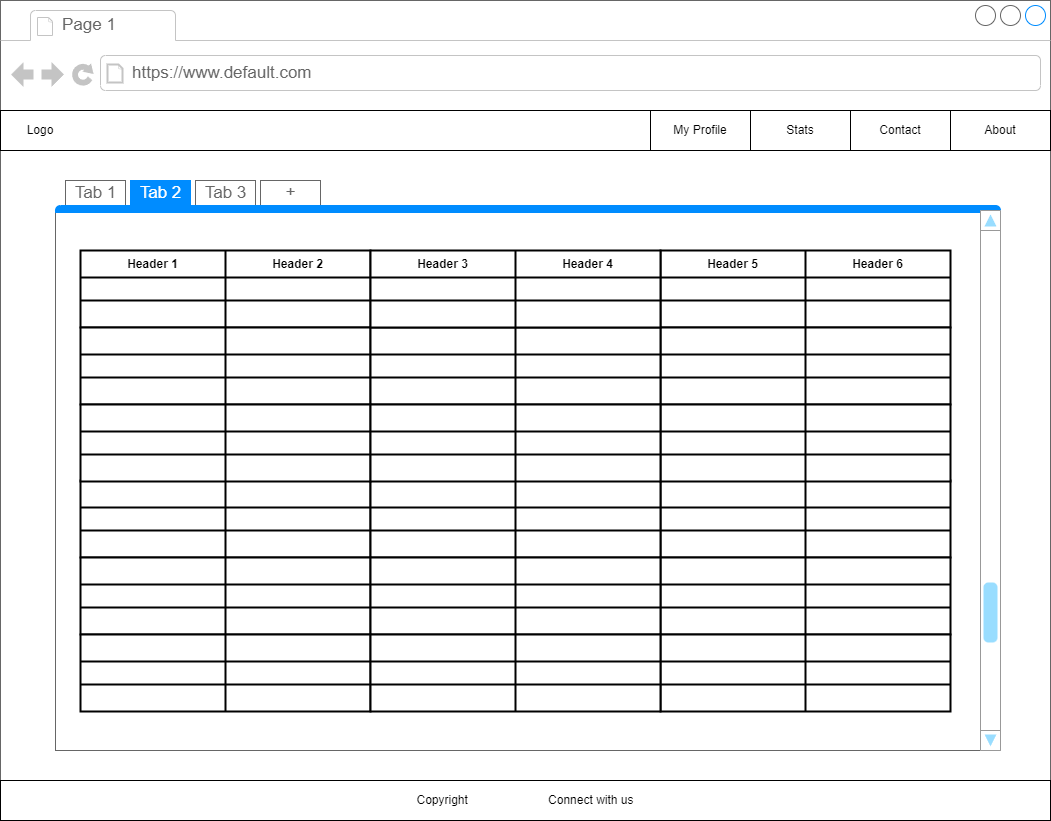
\includegraphics[width=0.6\textwidth]{loggedIn_starting_site}
    \caption{'Logged in' page}
\end{figure}

\begin{figure}[htbp]
    \centering
    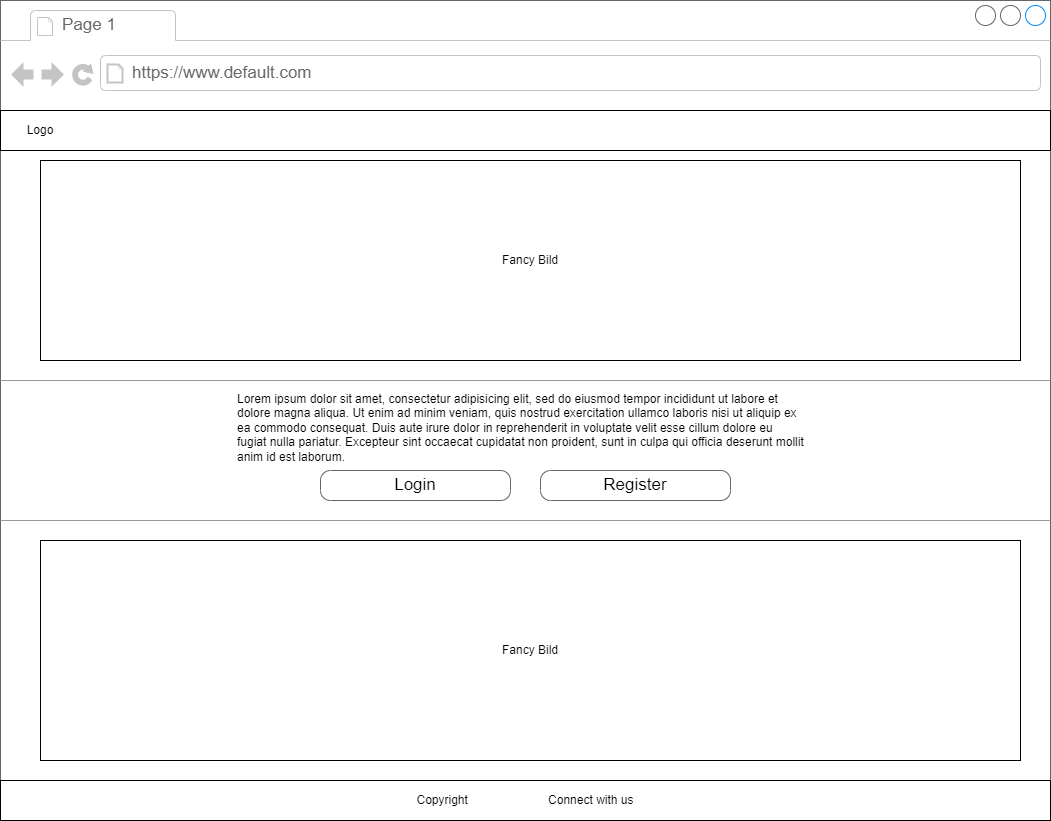
\includegraphics[width=0.6\textwidth]{Starting_site}
    \caption{Starting page}
\end{figure}


\end{document}